\documentclass[preprint2,numberedappendix,tighten,twocolappendix]{aastex6}  % USE THIS TO MAKE BIB, THEN FORMAT USING EMULATEAPJ
%\documentclass[twocolumn,apj,numberedappendix]{emulateapj}
\shorttitle{Data Analysis Methods for the Detection of the Epoch of Reionization}
\shortauthors{Cheng et al.}

\usepackage{amsmath}
\usepackage{graphicx}
\usepackage[figuresright]{rotating}
\usepackage{natbib}
\usepackage{ctable}
\citestyle{aa}

%		Math Shortcuts from Adrian
%\def\b{\mathbf{b}}
%\def\k{\mathbf{k}}
%\def\r{\mathbf{r}}
%\def\q{\mathbf{q}}
%\def\b{\mathbf{b}}
%\def\kp{\mathbf{k}^\prime}
%\def\kpp{\mathbf{k}^{\prime\prime}}
%\def\V{\mathbb{V}}
%\def\At{\tilde{A}}
%\def\Vt{\tilde{V}}
%\def\Tt{\tilde{T}}
%\def\tb{\langle T_b\rangle}
%\newcommand{\vis}{\mathbf{v}}
%\newcommand{\x}{\mathbf{x}}
%\newcommand{\xhat}{\hat{\mathbf{x}}}
%\newcommand{\nhat}{\hat{\mathbf{n}}}
%\newcommand{\A}{\mathbf{A}}
%\newcommand{\N}{\mathbf{N}}
%\newcommand{\rhat}{\hat{\mathbf{r}}}
%\newcommand{\khat}{\hat{\mathbf{k}}}
%\newcommand{\btheta}{\boldsymbol \theta}

\newcommand{\cc}[1]{{\color{purple} \textbf{[#1]}}}

\begin{document}
\title{Data Analysis Methods for the Detection of the Epoch of Reionization}

\author{
Carina Cheng\altaffilmark{1},
et al.
}


%		Notes	
	
%Reference section with: \ref{sec:Intro}
%Reference equation with: \eqref{eq:eqtest}
%Reference figure with: \ref{fig:figtest}
%Cite paper inside sentence: \citet{ref}
%Cite paper at end of sentence: \citep{ref}
%Cite paper inside a parenthetical sentence: \citealt{ref}

%To compile with references shown, compile in BibTeX once and LaTeX twice


%		Sample Equation Syntax
%\begin{equation}
%\label{eqtest}
%\langle \widetilde{T} (\mathbf{k}) \widetilde{T}^* (\mathbf{k^\prime}) \rangle = (2 \pi)^3 \delta^D (\mathbf{k} - \mathbf{k}^\prime) P(k),
%\end{equation}


\altaffiltext{1}{Astronomy Dept., U. California, Berkeley, CA}
%\altaffiltext{2}{Hubble Fellow}
%\altaffiltext{2}{Radio Astronomy Lab., U. California, Berkeley, CA}
%\altaffiltext{3}{Berkeley Center for Cosmological Physics, Berkeley, CA}
%\altaffiltext{3}{Dept. of Physics and Astronomy, U. Pennsylvania, Philadelphia, PA}
%\altaffiltext{8}{School of Earth and Space Exploration, Arizona State U., Tempe, AZ}

\begin{abstract}
The Epoch of Reionization (EoR) is an uncharted era in our Universe's history during which the birth of the first stars and galaxies led to the ionization of the omnipresent neutral hydrogen. This important epoch of our cosmic dawn harbors a wealth of information regarding the environment during this transformative time, including insight into the nature of the first luminous sources and implications about cosmological parameters. There are many experiments investigating the EoR by tracing the $21$ cm line of neutral hydrogen, a signal which is very faint and difficult to isolate. As instruments become more sensitive and a statistical power spectrum detection is in our foreseeable future, it has become increasingly important to develop techniques that help ensure that a potential detection isn't washed out or mistaken for something else. In this paper, we focus on two crucial ingredients for a power spectrum detection - a method for the accurate injection and recovery of an EoR signal, and jack-knife tests that can tease out foregrounds and systematics that contaminate our signal. We describe and apply these methods using data taken by the 64-element configuration of the Donald C. Baker Precision Array for Probing the Epoch of Reionization (PAPER).
\end{abstract}


\section{Introduction}
\label{sec:Intro}

By about one billion years after the Big Bang, the very first stars and galaxies are thought to have ionized all the neutral hydrogen that dominated the Universe's early life. This important transition, during which the first luminous structures formed from gravitational collapse and emit intense radiation, transforming the cold neutral gas into a plasma, is known as the epoch of reionization (EoR). The EoR represents an unexplored era in our cosmic dawn, whose history encodes important information regarding the nature of the first galaxies and the process of structure formation. A direct detection of the EoR would unlock powerful information about the intergalactic medium, revealing connections between the smooth matter distribution exhibited via cosmic microwave background (CMB) studies and the highly structured web of galaxies we observe today.

One promising technique to probe the EoR is to target the 21 cm wavelength emission that is emitted by neutral hydrogen via its spin-flip transition. This technique is powerful because it can be observed as a function of redshift - that is, the wavelength of the signal reaching our telescopes can be directly mapped to a distance from where the emission originated before stretching out as it traveled through expanding space. The 21 cm line therefore offers a window into following the evolution of ionization, temperature, and density fluctuations on cosmic scales.

Although a detection of the EoR has not currently been made to-date, there are several radio telescope experiments that have succeeded in using the 21 cm signal from hydrogen in order to place constraints on the brightness of the EoR. Examples of experiments investigating the mean brightness temperature of the EoR relative to the CMB are EDGES (\citealt{bowman2010}), the LWA (\citealt{ellingson_et_al2009}), LEDA (\citealt{greenhill_bernardi2012}), DARE (\citealt{burns2012}), SciHi (\citealt{voytek2014}), BIGHORNS (\citealt{sokolowski2015}), and SARAS (\citealt{patra2015}). Major interferometers, which seek to measure statistical power spectra, include the GMRT (\citealt{paciga_et_al2013}), LOFAR (\citealt{van_haarlem_et_al2013}), the MWA (\citealt{tingay_et_al2013}), the 21CMA (\citealt{peterson_et_al2004}, \citealt{wu2009}), and PAPER (\citealt{parsons_et_al2010}). The Hydrogen Epoch of Reionization Array (HERA), which is currently being built, is a next-generation instrument that hopes to combine lessons learned from previous experiments and is forecasted to be able to make a successful \cc{?$\sigma$} detection with an eventual \cc{?} elements.

The major challenge that faces all 21 cm experiments is in isolating a small signal that is buried underneath foregrounds and instrumental systematics that are 4-5 orders of magnitude brighter. A clean measurement therefore requires an intimate understanding of the instrument and a very careful, thorough understanding of data analysis choices. With HERA on the horizon and continual progress being made in the field, it is becoming increasingly more important to develop methods that can both reinforce a potential real detection and explain any false ones. In this paper, we present approaches to both of these issues using data from the 64-element configuration of PAPER. We place special emphasis on the accurate injection and recovery of a fake EoR signal in order to assess signal loss associated with different weighting techniques, as well as the importance of using jack-knife tests to investigate sources of bias.

This paper is organized as follows. In section 2 we give a brief overview of the PAPER-64 array and observations. In section 3 we describe our power spectrum estimation pipeline. Section 4 presents two key components of any power spectrum analysis pipeline - accurately quantifying signal loss that may result from data analysis choices, and choosing a weighting scheme to maximum foreground down-weighting without amassing large amounts of signal loss. In Section 5 we highlight useful jack-knife tests that can help discriminate between excess detections from foregrounds. We conclude in Section 6.

\section{Observations}
\label{sec:Obs}

The Donald C. Baker Precision Array for Probing the Epoch of Reionization (PAPER) is a dedicated 21 cm experiment located in the Karoo Desert in South Africa. The PAPER-64 configuration consists of 64 dual-polarization drift-scan elements, each 2 m on a side. The antenna layout is formatted in a grid layout (Figure \ref{fig:paper}), with 8 antennas on a side, 30 m spacing between antennas along the East/West direction, and 4 m spacing between antennas along the North/South direction. For the rest of this paper, we focus on data from only the 30 m pure East/West baselines. 

\begin{figure*}
	\centering
	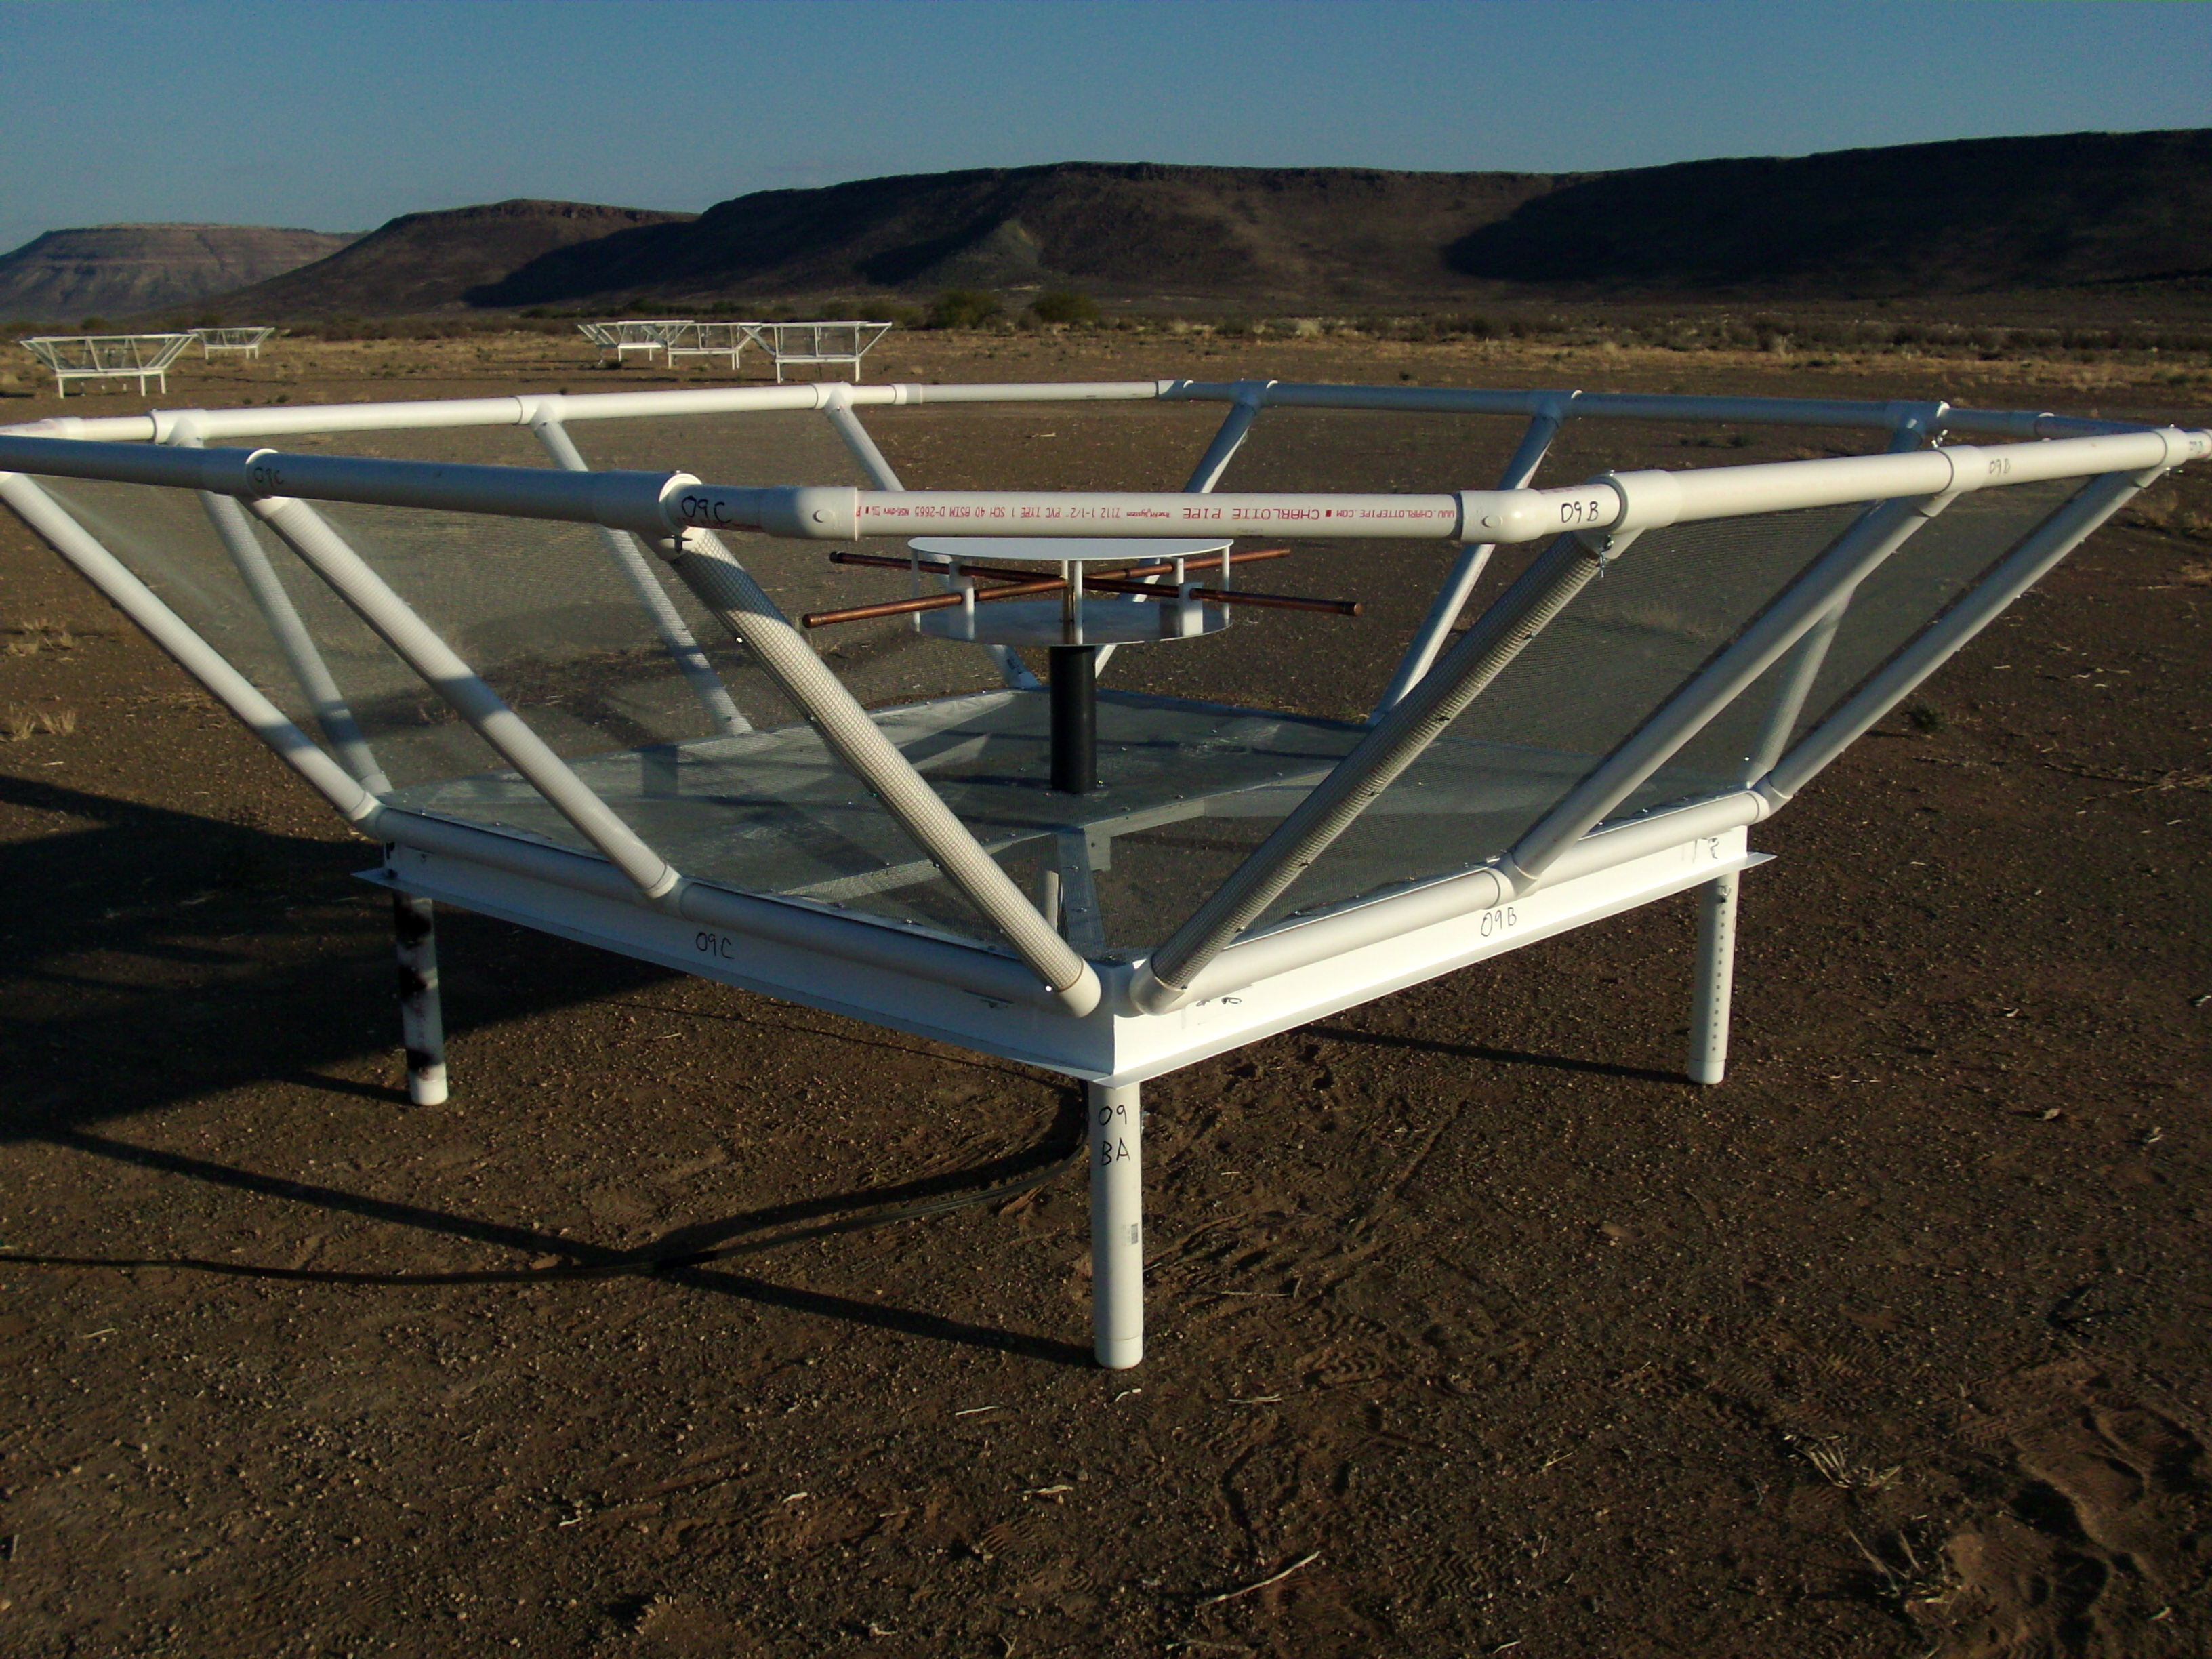
\includegraphics[height=0.35\textwidth]{paper_dipole.png}
	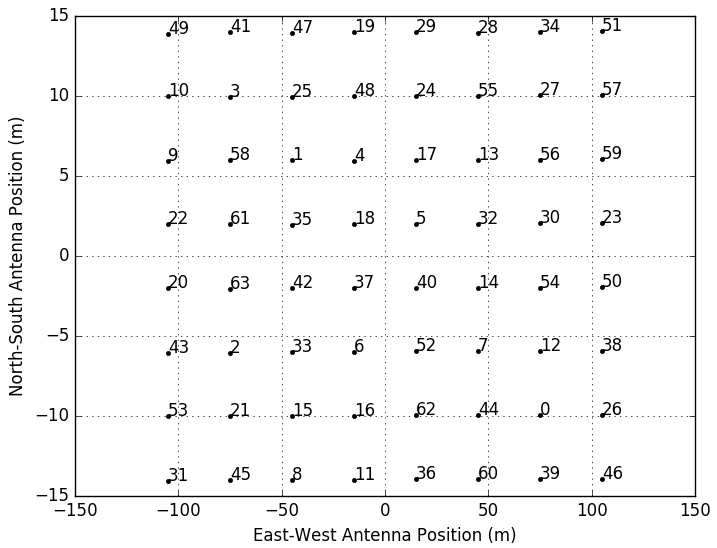
\includegraphics[height=0.35\textwidth]{antenna_layout.png}
	\caption{PAPER dipole in South Africa (left) and PAPER-64 antenna layout (right).}
	\label{fig:paper}
\end{figure*}

PAPER-64 observed for a total of 135 nights between 2012-2013. The correlator processes a bandwidth of 100-200 MHz, corresponding to a redshift range of 6-12. For more information about the backend system of PAPER-64 and its observations, we refer the reader to \cc{??} and \citet{ali_et_al2015}.

Because there is a detailed discussion of the PAPER-64 data reduction pipeline in \citet{ali_et_al2015}, here we will only briefly summarize the data processing steps prior to the power spectrum analysis. 

Beginning with compressed data products which have been cleaned of radio frequency interference (RFI) at the $6\sigma$ level and then down-sampled (to $42.9$ s integrations, $203$ frequency channels), we then employ the technique of redundant calibration as a means of calibrating for individual antenna gains without needing to use information about the sky. Because PAPER is laid out on a grid, antenna calibration parameters can be found through the use redundancy. Namely, baselines of the same length and orientation should measure the same sky signal, but in practice there are differences due to instrumental effects caused by antennas, cables, and receivers. Using the basis of redundancy, however, allows us to set up a system of equations to solve for a complex gain per antenna that brings all baseline of a particular type into alignment. We do this using the package OMNICAL.

We next solve for the array's overall phase and gain calibration parameters using a standard self calibration method. We used radio sources Pictor A, Fornax A, and the Crab Nebula to fit for an overall phase solution, and set our overall flux scale using Pictor A as a calibrator source. Although PAPER-64 data exists for all $4$ polarizations, we only use the $xx$ and $yy$ polarization data to form Stokes I as $V_{I} = \frac{1}{2}(V_{XX} + V_{YY})$.

Eliminating bright foregrounds remains a challenging yet crucial component of any 21 cm data analysis. There are many techniques to go about foreground removal, including spectral polynomial fitting, principle component analysis, Fourier-mode filtering, non-parametric subtractions, and inverse covariance weighting. PAPER uses a delay-spectrum filtering method which was first explained and applied in \citet{parsons_et_al2014}. In short, the delay-filtering technique employs the spectrally smooth nature of foregrounds, which are consequently localized in delay-space, the Fourier dual to frequency. We subtract all components that fall within the horizon limit for a specific baseline type in delay-space, plus a $15$ ns buffer, thus gaining about $\sim4$ orders of magnitude in sensitivity. 

Finally, after removing an additional layer of RFI (values $3\sigma$ above the median), we average together all our data into two datasets: even julian dates and odd julian dates. A total of $124$ nights of data comprises this average, and we use these two datasets as a starting point for constructing power spectrum estimates.

\section{Power Spectrum Analysis}
\label{sec:PS}

\subsection{Fringe-Rate-Filtering}
\label{sec:FRF}

As shown in \citet{parsons_et_al2016}, a fringe-rate filter allows us to maximize our sensitivity even further by averaging visibilities in time. We apply this filter in the fringe-rate domain, the Fourier-dual to time, and it effectively amounts to increasing our data's integration time. Another way to describe the filter is that it weights different parts of the sky (which rotate at different ``fringe-rates") by the antenna beam. This allows us to up-weight parts of the sky high in the primary beam, and down-weight those that are less sensitive.

In \citet{ali_et_al2015}, the filter applied was degraded (widened in fringe-rate space) from an optimal one that can be constructed based on the integration time of the data. This was chosen to decrease the resulting integration time, therefore increasing the number of independent modes and reducing signal loss associated with applying optimal quadratic estimators (OQE) on data with too few modes.

\begin{figure}
	\centering
	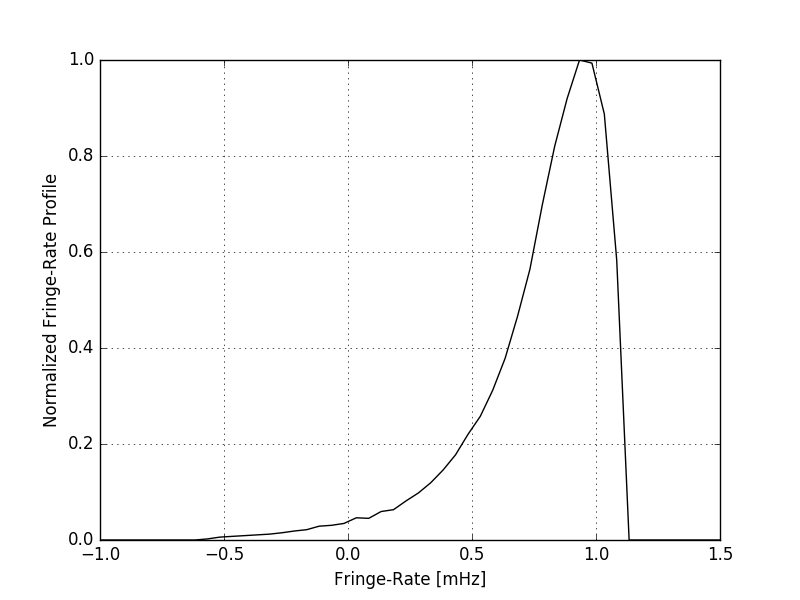
\includegraphics[width=\columnwidth]{frp.png}
	\caption{The optimal fringe-rate filter used in the analysis, normalized to $1$.}
	\label{fig:frp}
\end{figure}

New to our updated PAPER-64 analysis is the use of the optimal fringe-rate filter, which maximizes our sensitivity. With the development of a robust method for assessing signal loss (see Section \ref{sec:Sigloss}), we feel comfortable using a narrow filter (Figure \ref{fig:frp}), resulting in an effective integration time of $3857$ s (see Section \ref{sec:PSSense} for calculation) and $8$ total independent modes for our $8.5$ hours of LST. 

In practice, the optimal fringe-rate profile is computed for a fiducial $30$ m baseline at $150$ MHz, the center frequency in our band. The filter is implemented on a per baseline basis by convolving the time-domain visibilities with the Fourier transform of the fringe-rate filter, resulting in averaged visibilities yielding $\sim 2$ orders of magnitude in sensitivity.

\subsection{Power Spectrum Estimation}
\label{sec:PSEst}

To form power spectrum quantities using our two fringe-rate filtered, LST-binned datasets, we use OQE methods as described by \cc{??}. A summary of the method is as follows. 

We begin with our data vector $\textbf{x}$, which contains our visibilities that have the shape ($times$, $frequencies$) for each baseline and data group (`even' or `odd'). As part of our bootstrapping routine (and to speed things up), we divide up our total number of baselines into $5$ random, equal-sized groups, where no baselines are repeated within or between groups. For the \citet{ali_et_al2015} method, each group is then sampled with replacement to create a new group, of the same size, that can have repeated baselines inside it. We discover that in doing so, we are sacrificing some of our sensitivity since this results in there being 3-4 repeated baselines per group. In order to maximize our sensitivity but still apply random sampling for use in error estimation, we instead form new groups using all independent baselines except the very last one. For example, if we have $10$ baselines in a group, we use the first $9$ to guarantee at least $9$ independent measurements, and then fill the last slot randomly out of the $10$. We do this for all $5$ groups. This is still a valid means of bootstrapping because there are many more possibilities of baseline groupings than the number of bootstraps we run for this analysis ($nboots = 20$).

Taking $\textbf{x}$ to be averaged data from all baselines within a group, we now have $10$ possible data vectors (for $5$ groups and $2$ datasets). We next form the quantity $\hat{q}_{\alpha}$:

\begin{equation}
\hat{q}_{\alpha} = \frac{1}{2}\textbf{x}^{\dagger}\textbf{C}^{-1}\textbf{Q}_{\alpha}\textbf{C}^{-1}\textbf{x}-b_{\alpha}
\end{equation}

where $\textbf{C}$ is the covariance matrix defined to be $\textbf{C} \equiv \langle\textbf{x}\textbf{x}^{\dagger}\rangle$. The matrix $\textbf{Q}$ is an operator that takes our frequency-domain visibilities and Fourier-transforms them into power spectrum space. A noise bias $b_{\alpha}$ is subtracted off. The index $\alpha$ represents each $k_{\parallel}$ bin, where $k_{\parallel}$ is the Fourier-dual to frequency.

Notice that there are two quantities of $\textbf{C}^{-1}\textbf{x}$ in the expression for $\hat{q}$, representing two copies of inverse covariance weighted data. We perform all possible cross-multiplications of this quantity, except between the same datasets (`even' with `even', for example) and same groups (`baseline group 1' with `baseline group 1', for example). We avoid these computations to prevent the introduction of biases from shared auto power.

The rest of the OQE formalism is identical to \citet{ali_et_al2015}. We normalize our power spectrum estimates using the matrix $\textbf{M}$:

\begin{equation}
\hat{\textbf{p}} = \textbf{M}\hat{\textbf{q}}
\end{equation}

where $\hat{\textbf{p}}$ is the normalized estimate of the true power spectrum $\textbf{p}$. We compute $\textbf{M}$ using the Fisher matrix $\textbf{F}$, defined as:

\begin{eqnarray}
\textbf{F}_{\alpha\beta} &=& \frac{1}{2}tr(\textbf{C}^{-1}\textbf{Q}_{\alpha}\textbf{C}^{-1}\textbf{Q}_{\beta}). \\
\end{eqnarray}

We have a choice for $\textbf{M}$, and we choose to compute it by taking the Cholesky decomposition of $\textbf{F}$. Namely, we decompose the Fisher matrix such that $\textbf{F} = \textbf{L}\textbf{L}^{\dagger}$, where $\textbf{L}$ is a lower triangular matrix. Next, we construct $\textbf{M} = \textbf{D}\textbf{L}^{-1}$, where \textbf{D} is a diagonal matrix. Hence, our window function $\textbf{W} = \textbf{MF}$ becomes $\textbf{W} = \textbf{D}\textbf{L}^{\dagger}$ and is an upper triangular matrix. This window function was constructed in a way to prevent the leakage of foreground power from low $k$ to high $k$ modes. Specifically, we order the elements in $\textbf{F}$ in such a way so that power can leak from high $k$ modes to low $k$ modes, but not vice versa. Since most foreground power shows up at low $k$'s, this method ensures a window function that retains clean, noise-dominated measurements.

Finally, our final power spectrum is:

\begin{equation}
\hat{\textbf{p}} = \textbf{Wp}
\end{equation}

In practice, we end up with a 2-dimensional power spectrum quantity, which is a function of both time and $k$. We compute $20$ bootstraps of these quantities, where each bootstrap creates baseline groups randomly. 

In \citet{ali_et_al2015}, a second round of bootstrapping occurs over the bootstrap and time axes simultaneously. Random values are sampled with replacement along both axes, drawing as many values as there are number of bootstraps and times. Final power spectrum limits are then computed by taking the mean and standard deviation over this second bootstrap axis. 

However, we have found that this method greatly underestimates power spectrum errors, especially for fringe-rate filtered data. This can be explained by the fact that fringe-rate filtered data has a dramatically reduced number of independent modes. Hence, drawing $100$ samples out of a length-$100$ dataset that only has $5$ independent modes in it, for example, results in a narrower distribution of values that leads to a false error estimation.

To avoid this issue, we instead take a simple average along the time axis. Our final power spectrum limits are computed by taking the mean and standard deviation over our single bootstrap axis. 

In summary, our power spectrum pipeline begins with data with four axes (datasets, baselines, times, frequencies), bootstraps over baselines, uses OQE formalism, and produces $1$-dimensional power spectra for both $\textbf{P(k)}$ and the folded version $\Delta^{2}\textbf{(k)}$, defined as:

\begin{equation}
\Delta^{\textbf{2}}\textbf{(k)} = \frac{k^{3}}{2\pi^{2}}\hat{\textbf{p}}\textbf{(k)}
\end{equation}

One critical new component of our power spectrum pipeline is that we have many different power spectrum channels that simultaneously get processed at the same time and are especially useful for signal loss (Section \ref{sec:Sigloss}) and sensitivity (Section \ref{sec:Sense}) verification. Two important channels, in addition to our PAPER-64 data, are a noise dataset and an EoR dataset (in addition to these, we do different combinations of all three). We will briefly describe each.

We create random noise with a scale determined by the sensitivity of our instrument and parameters of our dataset. We calculate our system temperature for our frequencies of interest as:

\begin{equation}
T_{sys} = 180\Big(\frac{\nu}{0.18}\Big)^{-2.55} + T_{rcvr}
\end{equation}

where $\nu$ are frequencies in GHz. We use a receiver temperature of $200$ K, yielding $T_{sys} = 487$ at $150$ MHz. This is lower than in \citet{ali_et_al2015} because \cc{why?}. We convert this temperature into a variance statistic using:

\begin{equation}
T_{rms} = \frac{T_{sys}}{\sqrt{\Delta\nu \Delta t N_{days} N_{pols}}}
\end{equation}

where $\Delta\nu$ is channel spacing, $\Delta t$ is integration time, $N_{days}$ is the number of data samples for a particular time and frequency that went into our LST binned set, and $N_{pols}$ is the number of polarizations ($2$ for Stokes I). Our simulated noise has the same shape as our data, and we fringe-rate filter it in the same way to best mimic the real noise floor of our data. 

A second additional important channel in our pipeline is a simulated EoR signal. We again simulate random noise (with a default scale of $1$) with the same shape as our data, and we fringe-rate filter this signal twice. The first filter transforms the unattached noise into a signal that's attached to the sky (what our instrument observes). The second filter represents the fringe-rate filtering step in our data analysis pipeline. As described in Section \ref{sec:Sigloss}, we create an EoR signal at various amplitude levels.

Our multi-channel power spectrum pipeline has been essential in helping us understand the nuances in our pipeline. Because there are many different components and countless subtle effects affecting our final limits, it has been imperative to carry all our channels through the analysis to validate each step.

\subsection{Power Spectrum Sensitivity}
\label{sec:PSSense}

\cc{Add info on sensitivity equation, how we calculate effective inttime and adjust beam factor because of FRF, etc.}

\section{Signal Loss}
\label{sec:Sigloss}

\subsection{Formalism}
\label{sec:Formalism}

Based on our analysis pipeline, potential signal loss is a real and significant issue. More specifically, when applying inverse covariance weighting, $\textbf{C}^{-1}$ is empirically estimated from the data itself, which has the consequence of over-fitting the noise in the data, producing power spectra values well below the thermal noise limit that is predicted based on observation parameters. This is especially prevalent when weighting fringe-rate-filtered data, which has so few independent time modes to begin with, leading to a noisier dataset. Being able to accurately quantify this loss is crucial in interpreting and providing credibility to any power spectrum limits. 

New to the PAPER-64 analysis is a robust method to estimate signal loss associated with inverse covariance weighting. This method, explained below, is now a standard analysis step for all PAPER analyses and one that will be used for HERA moving forward.

As discussed previously, our power spectrum pipeline runs on a standardized set of channels (pure data, pure noise, pure EoR, and combinations of the three). As part of our signal loss routine, we also compute power spectra with various levels of the created EoR signal, dialing its amplitude from well-below the data level, to well-above. Suppose that $\textbf{e}$ is the injected EoR (at some amplitude level), and $\textbf{x}$ is our data vector. We define $\textbf{r}$ to be:

\begin{equation}
\textbf{r} = \textbf{x} + \textbf{e}
\end{equation}

Using our OQE formalism, we are interested in the following two quantities: $P_{in}$ and $P_{out}$. The input power spectrum, $P_{in}$ represents the unweighted power spectrum of only $\textbf{e}$, our simulated EoR signal. The output power spectrum, $P_{out}$, is the weighted power spectrum of $\textbf{e}$ that would result from our pipeline if the signal was mixed with our data. Comparing the two quantities yields insight into how much of $\textbf{e}$ is lost due to our choice of weighting. Ignoring normalization, factors:

\begin{equation}
P_{in} \propto \textbf{e}^{\dagger}\textbf{I}^{-1}\textbf{Q}\textbf{I}^{-1}\textbf{e}
\end{equation}

\begin{eqnarray}
\label{eq:sigloss}
P_{out} \equiv \textbf{P}_{e} &=& \textbf{P}_{r}-\textbf{P}_{x} \nonumber \\
&\propto& \textbf{r}^{\dagger}\textbf{C}_{r}^{-1}\textbf{Q}\textbf{C}_{r}^{-1}\textbf{r} - \textbf{x}^{\dagger}\textbf{C}_{x}^{-1}\textbf{Q}\textbf{C}_{x}^{-1}\textbf{x} 
\end{eqnarray}

It is noted that the output power spectrum is comprised of two terms: the covariance treated power spectrum associated with \textbf{r}, and that of data \textbf{x} alone. 

One may wonder why $P_{out}$ cannot be computed simply as the weighted power spectrum of $\textbf{e}$ alone, namely $P_{out} \propto \textbf{e}^{\dagger}\textbf{C}_{e}^{-1}\textbf{Q}\textbf{C}_{e}^{-1}\textbf{e}$. Expanding Equation \ref{eq:sigloss}:

\begin{eqnarray}
P_{out} &\propto& (\textbf{x}+\textbf{e})^{\dagger}\textbf{C}_{r}^{-1}\textbf{Q}\textbf{C}_{r}^{-1}(\textbf{x}+\textbf{e}) - \textbf{x}^{\dagger}\textbf{C}_{x}^{-1}\textbf{Q}\textbf{C}_{x}^{-1}\textbf{x} \nonumber \\
&\propto& \textbf{x}^{\dagger}\textbf{C}_{r}^{-1}\textbf{Q}\textbf{C}_{r}^{-1}\textbf{x} + \textbf{e}^{\dagger}\textbf{C}_{r}^{-1}\textbf{Q}\textbf{C}_{r}^{-1}\textbf{e} + \textbf{x}^{\dagger}\textbf{C}_{r}^{-1}\textbf{Q}\textbf{C}_{r}^{-1}\textbf{e} \nonumber \\
&+& \textbf{e}^{\dagger}\textbf{C}_{r}^{-1}\textbf{Q}\textbf{C}_{r}^{-1}\textbf{x} - \textbf{x}^{\dagger}\textbf{C}_{x}^{-1}\textbf{Q}\textbf{C}_{x}^{-1}\textbf{x} \nonumber 
\end{eqnarray}

And taking the case of very large $\textbf{e}$, so that $\textbf{C}_{r}^{-1} \sim \textbf{C}_{e}^{-1}$ and any terms involving only $\textbf{x}$ are small:

\begin{eqnarray}
P_{out, \textbf{e} \gg \textbf{x}} &\propto& \textbf{e}^{\dagger}\textbf{C}_{e}^{-1}\textbf{Q}\textbf{C}_{e}^{-1}\textbf{e} + \textbf{x}^{\dagger}\textbf{C}_{e}^{-1}\textbf{Q}\textbf{C}_{e}^{-1}\textbf{e} \nonumber \\
&+& \textbf{e}^{\dagger}\textbf{C}_{e}^{-1}\textbf{Q}\textbf{C}_{e}^{-1}\textbf{x}
\end{eqnarray}

We see that our naive expression for $P_{out}$ is the first term, but there also two additional terms. An initial assumption would be that the cross-terms that involve both $\textbf{e}$ and $\textbf{x}$ should be zero, since the two quantities are un-correlated. However, \cc{need explanation about power in cross-terms here}. Therefore, in our investigation of signal loss, we use the full quantity for $P_{out}$ as in Equation \ref{eq:sigloss}.

For the unweighted case ($\textbf{C} \equiv \textbf{I}$), we expect $P_{out}$ and $P_{in}$ to be equal, and hence the ratio of $P_{in} / P_{out}$ to be 1. For the weighted case, this is not true due to signal loss. In order to quantify the loss, we look at the ratio of $P_{in}$ to $P_{out}$ as the amplitude level of the injected signal \textbf{e} is increased. In the next section, we highlight two methods that yield similar results for the determination of signal loss using $P_{in}$ and $P_{out}$

\subsection{Application}
\label{sec:siglossprac}

Recall that fringe-rate filtered noise, which mimics the level of noise in our actual PAPER-64 dataset, is a channel in our power spectrum pipeline. We can compute signal loss quantities of interest for the noise $\textbf{n}$ similar to the expressions we featured previously for data $\textbf{x}$. 

\begin{eqnarray}
P_{in} &\propto& \textbf{e}^{\dagger}\textbf{I}^{-1}\textbf{Q}\textbf{I}^{-1}\textbf{e} \\
\textbf{s} &=& \textbf{n} + \textbf{e} \\
P_{out} &\propto& \textbf{s}^{\dagger}\textbf{C}_{s}^{-1}\textbf{Q}\textbf{C}_{s}^{-1}\textbf{s} - \textbf{n}^{\dagger}\textbf{C}_{n}^{-1}\textbf{Q}\textbf{C}_{n}^{-1}\textbf{n} 
\end{eqnarray}

Using the input and output power spectra for range of EoR amplitudes, we use two methods to determine signal loss associated with the over-fitting of noise during inverse covariance weighting. We first look at signal loss for the pure noise case (no data), to show that we can successfully inject EoR signals, determine signal loss, and then recover the signal.

The first method is very straightforward. Post-bootstrapping, our final power spectra are 1-dimensional and only a function of $k$. For each $k$, we simply look at $P_{out}$ as a function of $P_{in}$, as shown in Figure \ref{fig:sigloss1_noise}. The shape of this function can be explained as follows. At small injection levels (small $\textbf{e}$), $P_{out}$ and $P_{in}$ are equal, and there is no signal loss. As the amplitude of EoR increases, we then move into a regime where the final output power spectrum is lower than the unweighted input one. This is dangerous, because without correcting for this effect one might be led to underestimate the EoR signal. The peculiar tail at very low injection levels (where $P_{out} > P_{in}$) is an unphysical feature, but rather illustrates that there is some non-negligible cross-term power between $\textbf{n}$ and $\textbf{e}$.

For this method, we interpolate the signal loss factor (per $k$), computed as $P_{in}/P_{out}$, at a $P_{out}$ value equal to the $2\sigma$ power spectrum upper limit of noise alone. In other words, we look at $P_{noise} \propto \textbf{n}^{\dagger}\textbf{C}_{n}^{-1}\textbf{Q}\textbf{C}_{n}^{-1}\textbf{n}$, compute its $2\sigma$ upper limit (mean over bootstraps + $2 \times $standard deviation over bootstraps), and interpolate the value of $P_{in}/P_{out}$ at this value. We therefore end up with one signal loss correction factor per $k$. 

\begin{figure*}
	\centering
	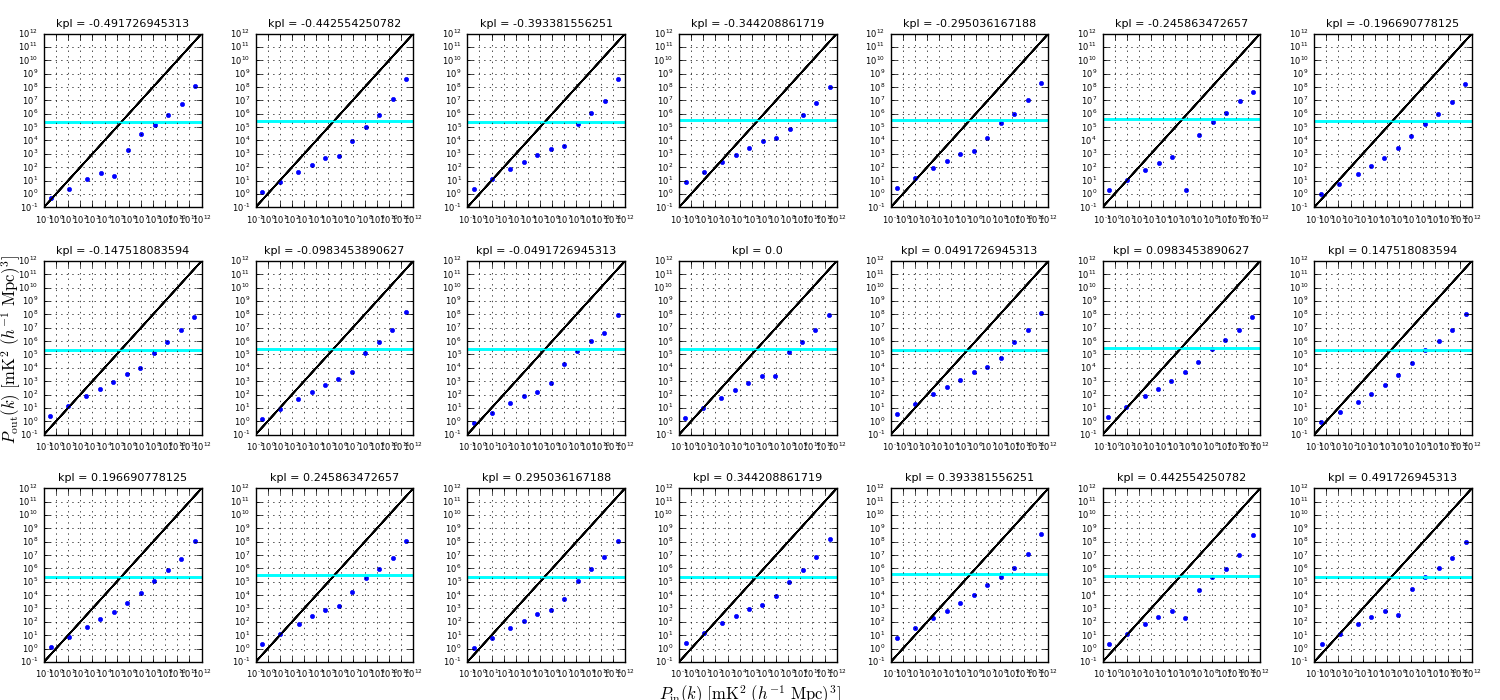
\includegraphics[width=1.0\textwidth]{sigloss1_noise.png}
	\caption{$P_{in}$ vs. $P_{out}$ (blue points) for 15 injection levels and 21 $k$'s. The solid cyan line is the $2\sigma$ upper limit for the weighted power spectrum of noise alone, and it is at this level where the signal loss factor $P_{in}/P_{out}$ is computed by interpolation. \cc{Maybe re-do this plot with closer-together points}}
	\label{fig:sigloss1_noise}
\end{figure*}

Figure \ref{fig:ps1_noise} shows the power spectrum of our noise simulation, using full inverse covariance weighting, both before and after signal loss correction. Prior to signal loss correction, it is obvious that the power spectrum is unfeasible because it is well below the theoretical noise level prediction. Post-correction, the power spectrum values blow up much higher than both the theory and unweighted power spectrum. This is an effect caused by the steep nature of the eigenspectrum of $\textbf{C}$, and is explained more in Section \ref{sec:Weight}.

\cc{Need a plot that shows our signal loss factors are CORRECT. How to do that??}

\begin{figure*}
	\centering
	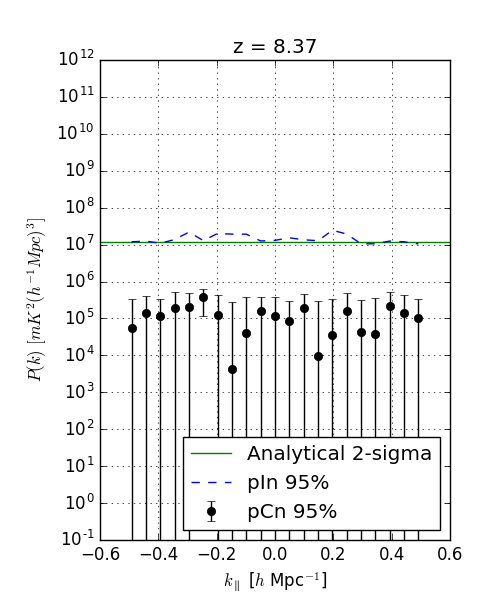
\includegraphics[width=0.4\textwidth]{ps1_noise_nosigloss.png}
	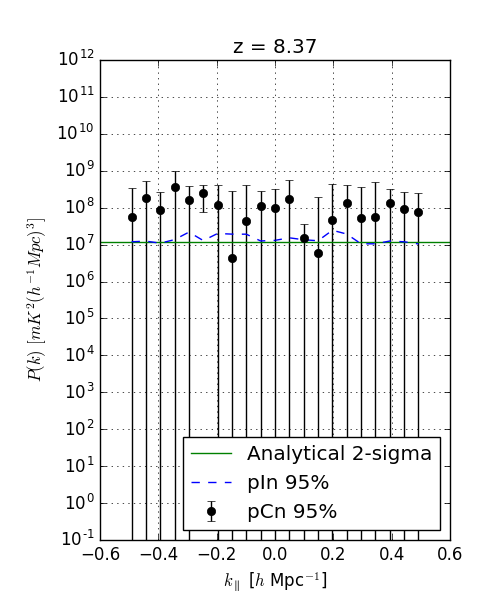
\includegraphics[width=0.4\textwidth]{ps1_noise.png}
	\caption{Full inverse covariance weighted power spectrum of pure noise (black points, with $2\sigma$ error bars) before signal loss correction (left) and after (right). The dashed blue line is the unweighted power spectrum ($2\sigma$ upper limit). The solid green line is the theoretical noise level prediction based on observational parameters. \cc{Color negative points grey}}
	\label{fig:ps1_noise}
\end{figure*}

Our second method for estimating signal loss is similar to the first, but more comprehensive in a statistical sense. Instead of looking at input and output power spectra after bootstrapping, we now look at their values for every bootstrap in order to get a sense of their distributions. Figure \ref{fig:sigloss2_noise} plots $P_{in}$ vs. $P_{out}$ for $20$ bootstraps, and as expected, the function now has a spread in the width-direction in comparison to what was plotted in Figure \ref{fig:sigloss1_noise}, but otherwise shows a familiar trend. Similarly, our weighted noise power spectra also has a defined spread due to bootstrapping.

Using these two distributions ($P_{in}/P_{out}$ and $P_{noise}$), we can create bins along the $P_{noise}$ axis to yield histograms of signal loss factors for each bin. We similarly sort the values of $P_{noise}$ into the same bins, and multiply the probability of $P_{noise}$ per bin (the number of values falling into that bin, divided by the total) with the signal loss factors in that bin, essentially computing a weighted average across all bins to obtain a final signal loss factor per $k$. As shown in Figure \ref{fig:ps2_noise}, the results are very similar to the previous method. For future power spectrum results, we choose to use the second method because it computes final signal loss values using our full distributions of measurements.

One thing to note is that for both methods, we have been careful to validate that the computations yield no signal loss (signal loss factors of $1$) for the unweighted power spectrum case, as is expected. This is important in confirming that signal loss is a direct result of the choice for $\textbf{C}$.

\begin{figure*}
	\centering
	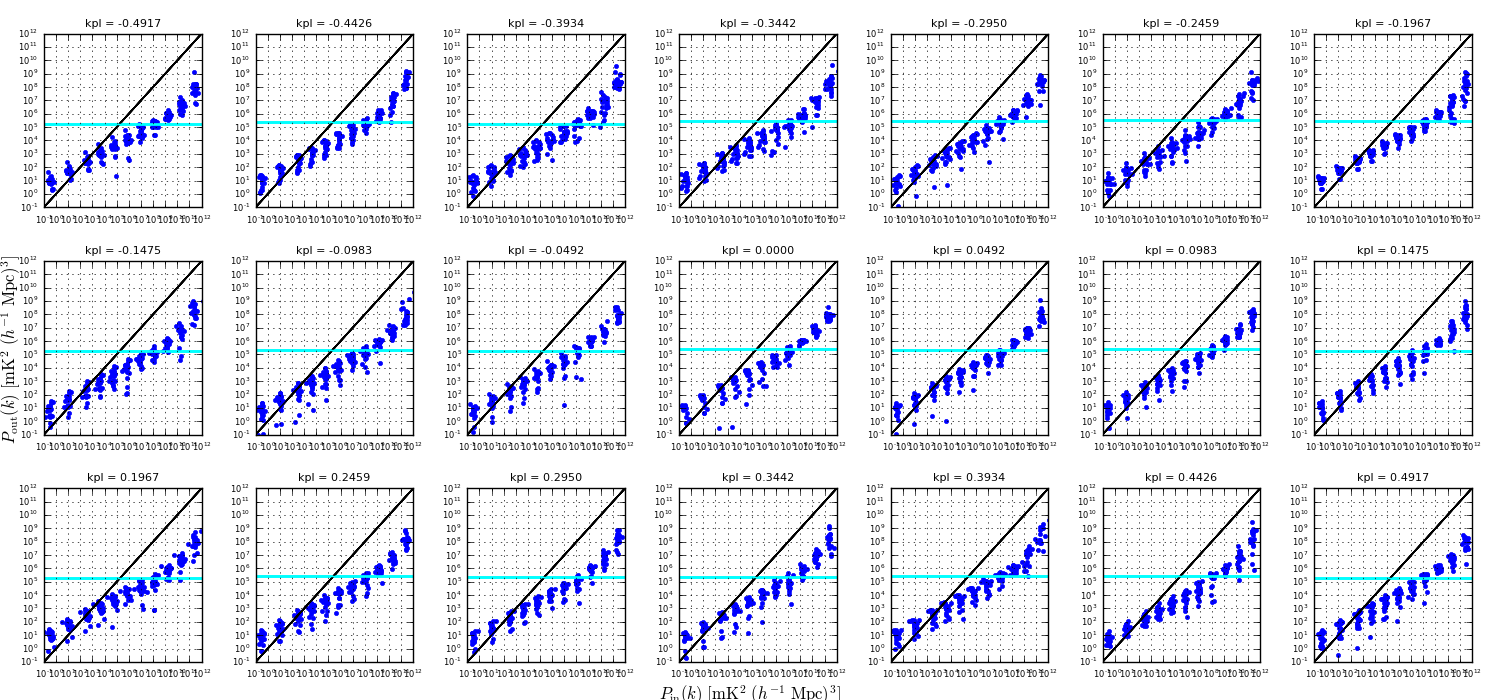
\includegraphics[width=1.0\textwidth]{sigloss2_noise.png}
	\caption{$P_{in}$ vs. $P_{out}$ (blue) for 15 injection levels, 20 bootstraps, and 21 $k$'s. \cc{Plot a semi-transparent cyan range of pCn values instead of just the max}}
	\label{fig:sigloss2_noise}
\end{figure*}

\begin{figure*}
	\centering
	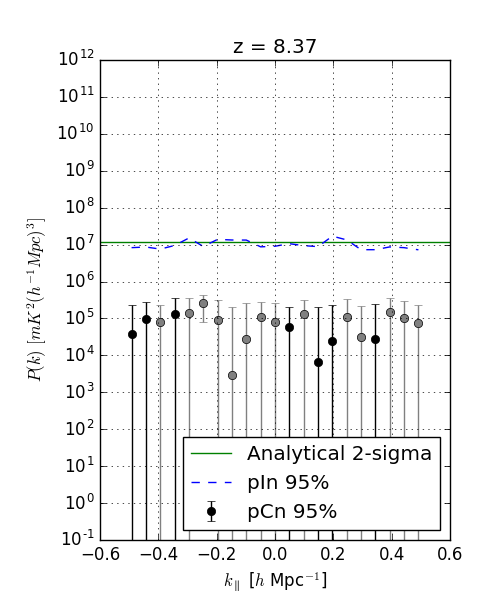
\includegraphics[width=0.4\textwidth]{ps2_noise_nosigloss.png}
	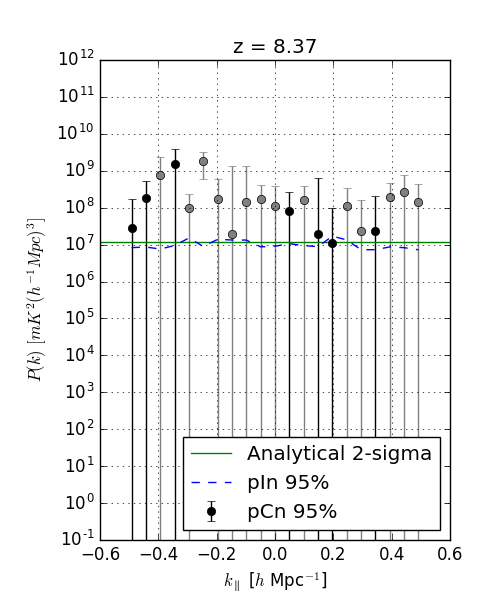
\includegraphics[width=0.4\textwidth]{ps2_noise.png}
	\caption{Full inverse covariance weighted power spectrum of pure noise (black and grey points, with $2\sigma$ error bars) before signal loss correction (left) and after (right). Black points correspond to positive values, while grey points correspond to originally negative values that have been made positive for plotting. The dashed blue line is the unweighted power spectrum ($2\sigma$ upper limit). The solid green line is the theoretical noise level prediction based on observational parameters.}
	\label{fig:ps2_noise}
\end{figure*}

\subsection{Data Weighting}
\label{sec:Weight}

With our signal loss formalism established, we now have the capability of experimenting with different weighting options for $\textbf{C}$. Our goal here is to choose a weighting method that successfully down-weights foregrounds and systematics in our data without generating large amounts of signal loss. We have found that the balance between the two is a delicate one and requires \cc{?? finish sentence...}. 

We now turn our attention to power spectra using the 30 m East/West baselines of PAPER-64. Our dataset spans $8.5$ hours of LST ($.1$-$8.6$ hrs), includes a total of $51$ baselines, and is fringe-rate filtered using an optimal fringe-rate filter. We have two datasets (even days and odd days), and only cross-multiply data from different days and different baselines. We are interested in $21$ frequency channels (channels 95-115), which yields a power spectrum for a redshift of $z=8.4$. 

Using full inverse covariance weighting, our results are not too dissimilar to that of pure noise. Signal loss factors (Figure \ref{fig:sigloss2_data}) are of similar order of magnitude, and our power spectrum blows up past the unweighted version after signal loss correction (Figure \ref{fig:ps2_data}).

%\begin{figure*}
%	\centering
%	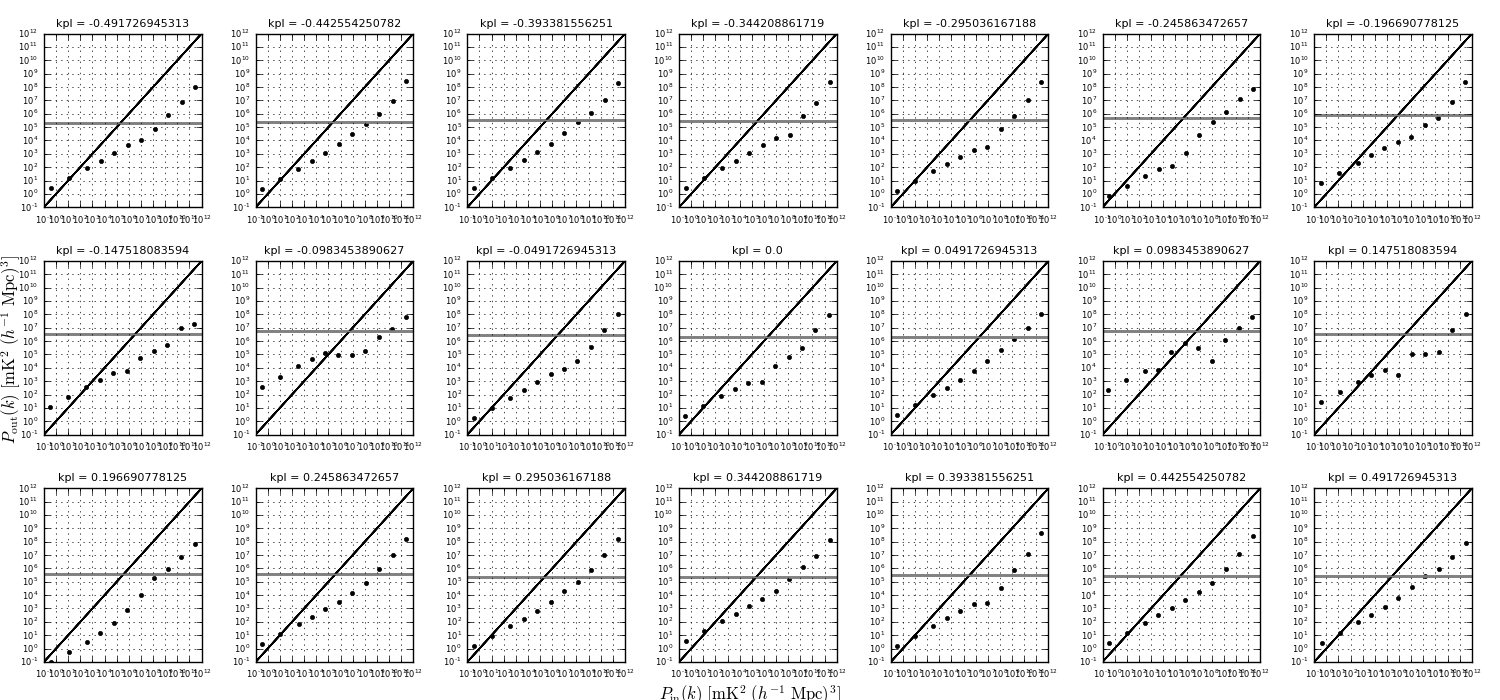
\includegraphics[width=1.0\textwidth]{sigloss1_data.png}
%	\caption{$P_{in}$ vs. $P_{out}$ (black) for 15 injection levels and 21 $k$'s. The solid grey line is the $2\sigma$ upper limit for the weighted power spectrum of data alone, and it is at this level where the signal loss factor $P_{in}/P_{out}$ is computed by interpolation. \cc{Probably don't need to show this plot at all}}
%	\label{fig:sigloss1_data}
%\end{figure*}

\begin{figure*}
	\centering
	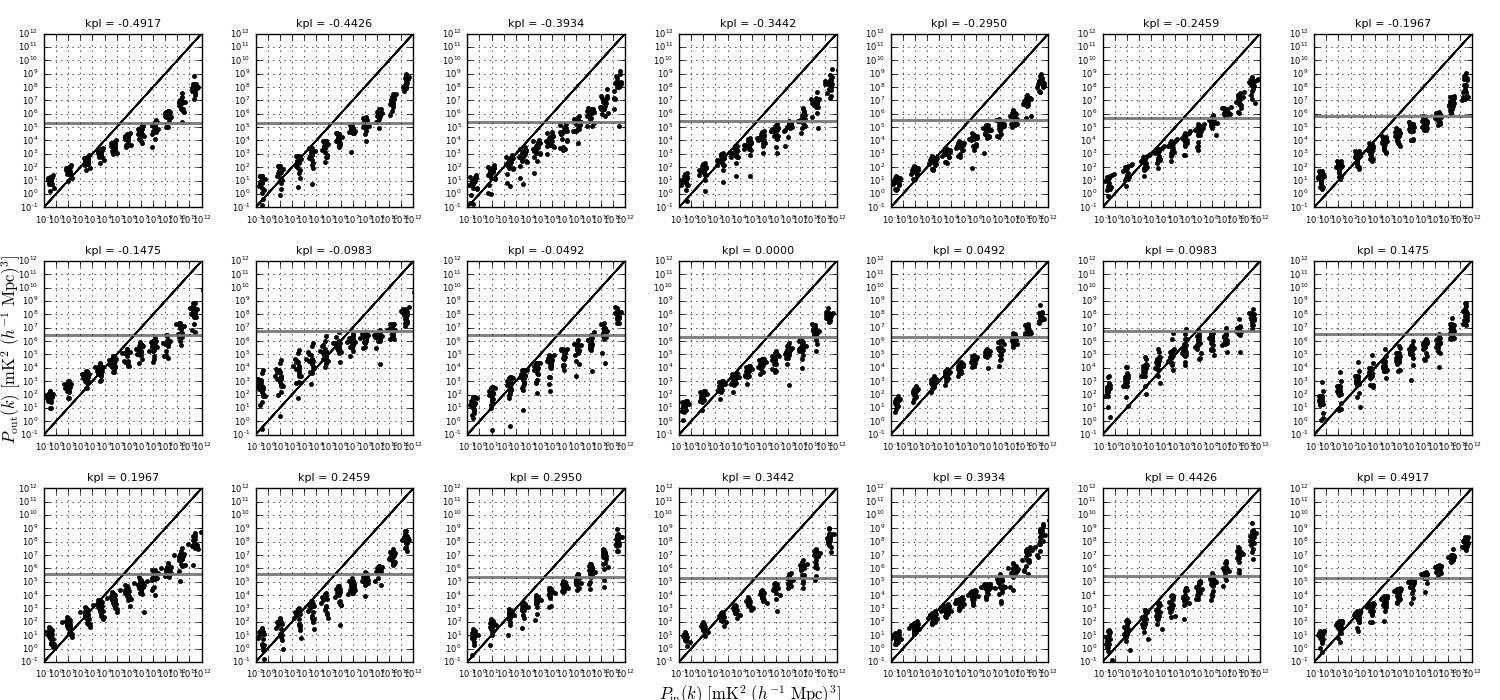
\includegraphics[width=1.0\textwidth]{sigloss2_data.png}
	\caption{$P_{in}$ vs. $P_{out}$ (black) for 15 injection levels, 20 bootstraps, and 21 $k$'s. \cc{Plot a semi-transparent grey range of pCv values instead of just the max}}
	\label{fig:sigloss2_data}
\end{figure*}

\begin{figure*}
	\centering
	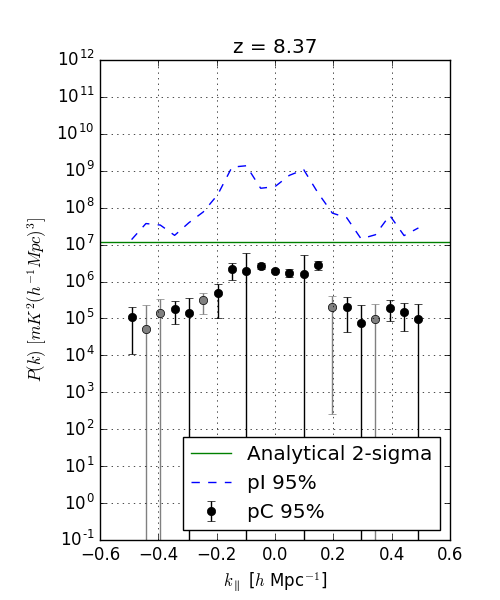
\includegraphics[width=0.4\textwidth]{ps2_data_nosigloss.png}
	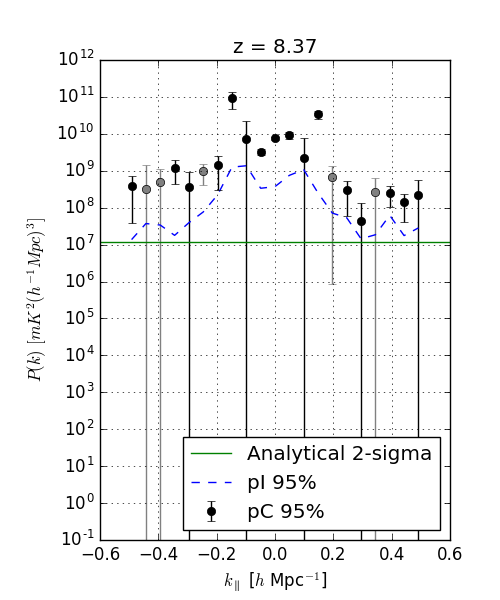
\includegraphics[width=0.4\textwidth]{ps2_data.png}
	\caption{Full inverse covariance weighted power spectrum of PAPER-64 data (black and grey points, with $2\sigma$ error bars) before signal loss correction (left) and after (right). Black points correspond to positive values, while grey points correspond to originally negative values that have been made positive for plotting. The dashed blue line is the unweighted power spectrum ($2\sigma$ upper limit). The solid green line is the theoretical noise level prediction based on observational parameters.}
	\label{fig:ps2_data}
\end{figure*}

Looking into this behavior in more detail, we investigate the shape of the eigenspectrum of $\textbf{C}$ for a typical baseline used in the analysis. Figure \ref{fig:eigenspectrum} shows this spectrum for baseline (1,4). Most obviously, the spectrum is steep, spanning 4 orders of magnitude. Not as obvious is the effect of this shape on our results. When the matrix $\textbf{C}$ is inverted to form $\textbf{C}^{-1}$, the effect of the steepness of the eigenspectrum is to up-weight very few modes of the sky while the rest are drastically down-weighted. More specifically, our fringe-rate filtered data contains a finite, small number of independent modes, thereby resulting in a covariance matrix that can be described by just a few modes. Beyond the first few modes, the eigenvalues of each additional mode falls of dramatically. When inverting, we end up not only down-weighting those initial modes but severely up-weighting a few insignificant ones. Because of our weighting choice, signal loss blows up as it thinks we only have a couple modes in our data.

\begin{figure*}
	\centering
	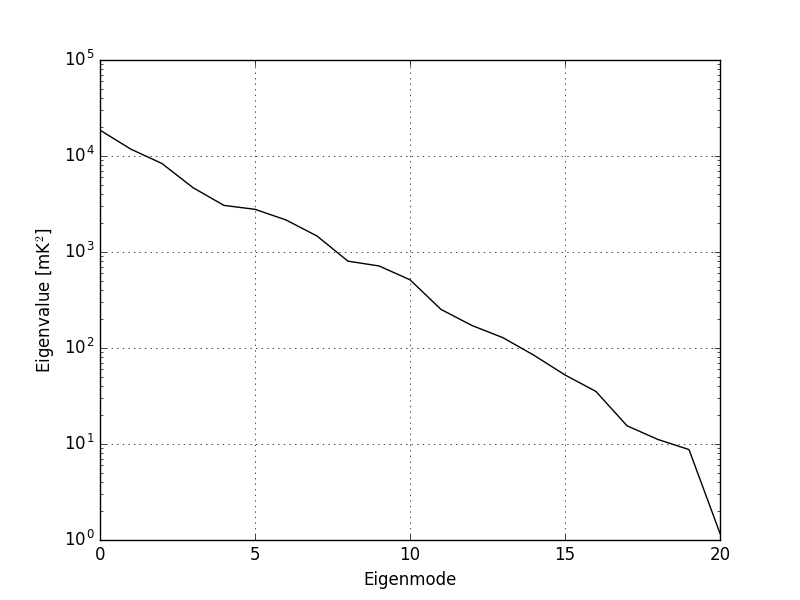
\includegraphics[width=0.4\textwidth]{eigenspectrum.png}
	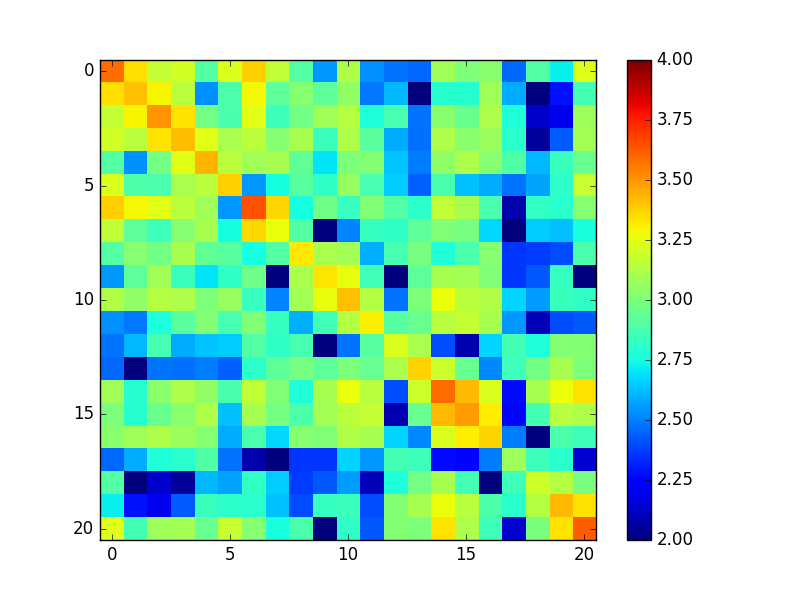
\includegraphics[width=0.4\textwidth]{covariance.png}
	\caption{Eigenspectrum for $\textbf{C}$ for baseline (1,4) for the 21 channels ofs interest (left) and covariance matrix $\textbf{C}$ for the same baseline (right).}
	\label{fig:eigenspectrum}
\end{figure*}

Clearly the full inverse covariance treatment of our data is suboptimal to even the unweighted case, but we would like to find a weighting method that does successfully down-weight contaminants in our data and make some improvement over the unweighted power spectrum. There are many choices for determining the covariance matrix $\textbf{C}$, but here we will illustrate \cc{?} promising ones as applied to PAPER-64.

\cc{TO DO: decide on/explain/show different weightings}

\section{Jack-Knives}
\label{sec:Jack}

\section{Conclusion}
\label{sec:Con}

\section{Acknowledgements}
\cc{NSF Graduate Research Fellowship Program (GRFP) Fellowship}
\cc{UC Berkeley Chancellor's Fellowship}
\label{sec:Ack}

\bibliographystyle{apj}
\bibliography{refs}


\end{document}

